\PassOptionsToPackage{unicode=true}{hyperref} % options for packages loaded elsewhere
\PassOptionsToPackage{hyphens}{url}
%
\documentclass[]{book}
\usepackage{lmodern}
\usepackage{amssymb,amsmath}
\usepackage{ifxetex,ifluatex}
\usepackage{fixltx2e} % provides \textsubscript
\ifnum 0\ifxetex 1\fi\ifluatex 1\fi=0 % if pdftex
  \usepackage[T1]{fontenc}
  \usepackage[utf8]{inputenc}
  \usepackage{textcomp} % provides euro and other symbols
\else % if luatex or xelatex
  \usepackage{unicode-math}
  \defaultfontfeatures{Ligatures=TeX,Scale=MatchLowercase}
\fi
% use upquote if available, for straight quotes in verbatim environments
\IfFileExists{upquote.sty}{\usepackage{upquote}}{}
% use microtype if available
\IfFileExists{microtype.sty}{%
\usepackage[]{microtype}
\UseMicrotypeSet[protrusion]{basicmath} % disable protrusion for tt fonts
}{}
\IfFileExists{parskip.sty}{%
\usepackage{parskip}
}{% else
\setlength{\parindent}{0pt}
\setlength{\parskip}{6pt plus 2pt minus 1pt}
}
\usepackage{hyperref}
\hypersetup{
            pdftitle={An RNA-seq Data Analysis Protocol},
            pdfauthor={David Chisanga and Wei Shi},
            pdfborder={0 0 0},
            breaklinks=true}
\urlstyle{same}  % don't use monospace font for urls
\usepackage{color}
\usepackage{fancyvrb}
\newcommand{\VerbBar}{|}
\newcommand{\VERB}{\Verb[commandchars=\\\{\}]}
\DefineVerbatimEnvironment{Highlighting}{Verbatim}{commandchars=\\\{\}}
% Add ',fontsize=\small' for more characters per line
\usepackage{framed}
\definecolor{shadecolor}{RGB}{248,248,248}
\newenvironment{Shaded}{\begin{snugshade}}{\end{snugshade}}
\newcommand{\AlertTok}[1]{\textcolor[rgb]{0.94,0.16,0.16}{#1}}
\newcommand{\AnnotationTok}[1]{\textcolor[rgb]{0.56,0.35,0.01}{\textbf{\textit{#1}}}}
\newcommand{\AttributeTok}[1]{\textcolor[rgb]{0.77,0.63,0.00}{#1}}
\newcommand{\BaseNTok}[1]{\textcolor[rgb]{0.00,0.00,0.81}{#1}}
\newcommand{\BuiltInTok}[1]{#1}
\newcommand{\CharTok}[1]{\textcolor[rgb]{0.31,0.60,0.02}{#1}}
\newcommand{\CommentTok}[1]{\textcolor[rgb]{0.56,0.35,0.01}{\textit{#1}}}
\newcommand{\CommentVarTok}[1]{\textcolor[rgb]{0.56,0.35,0.01}{\textbf{\textit{#1}}}}
\newcommand{\ConstantTok}[1]{\textcolor[rgb]{0.00,0.00,0.00}{#1}}
\newcommand{\ControlFlowTok}[1]{\textcolor[rgb]{0.13,0.29,0.53}{\textbf{#1}}}
\newcommand{\DataTypeTok}[1]{\textcolor[rgb]{0.13,0.29,0.53}{#1}}
\newcommand{\DecValTok}[1]{\textcolor[rgb]{0.00,0.00,0.81}{#1}}
\newcommand{\DocumentationTok}[1]{\textcolor[rgb]{0.56,0.35,0.01}{\textbf{\textit{#1}}}}
\newcommand{\ErrorTok}[1]{\textcolor[rgb]{0.64,0.00,0.00}{\textbf{#1}}}
\newcommand{\ExtensionTok}[1]{#1}
\newcommand{\FloatTok}[1]{\textcolor[rgb]{0.00,0.00,0.81}{#1}}
\newcommand{\FunctionTok}[1]{\textcolor[rgb]{0.00,0.00,0.00}{#1}}
\newcommand{\ImportTok}[1]{#1}
\newcommand{\InformationTok}[1]{\textcolor[rgb]{0.56,0.35,0.01}{\textbf{\textit{#1}}}}
\newcommand{\KeywordTok}[1]{\textcolor[rgb]{0.13,0.29,0.53}{\textbf{#1}}}
\newcommand{\NormalTok}[1]{#1}
\newcommand{\OperatorTok}[1]{\textcolor[rgb]{0.81,0.36,0.00}{\textbf{#1}}}
\newcommand{\OtherTok}[1]{\textcolor[rgb]{0.56,0.35,0.01}{#1}}
\newcommand{\PreprocessorTok}[1]{\textcolor[rgb]{0.56,0.35,0.01}{\textit{#1}}}
\newcommand{\RegionMarkerTok}[1]{#1}
\newcommand{\SpecialCharTok}[1]{\textcolor[rgb]{0.00,0.00,0.00}{#1}}
\newcommand{\SpecialStringTok}[1]{\textcolor[rgb]{0.31,0.60,0.02}{#1}}
\newcommand{\StringTok}[1]{\textcolor[rgb]{0.31,0.60,0.02}{#1}}
\newcommand{\VariableTok}[1]{\textcolor[rgb]{0.00,0.00,0.00}{#1}}
\newcommand{\VerbatimStringTok}[1]{\textcolor[rgb]{0.31,0.60,0.02}{#1}}
\newcommand{\WarningTok}[1]{\textcolor[rgb]{0.56,0.35,0.01}{\textbf{\textit{#1}}}}
\usepackage{longtable,booktabs}
% Fix footnotes in tables (requires footnote package)
\IfFileExists{footnote.sty}{\usepackage{footnote}\makesavenoteenv{longtable}}{}
\usepackage{graphicx,grffile}
\makeatletter
\def\maxwidth{\ifdim\Gin@nat@width>\linewidth\linewidth\else\Gin@nat@width\fi}
\def\maxheight{\ifdim\Gin@nat@height>\textheight\textheight\else\Gin@nat@height\fi}
\makeatother
% Scale images if necessary, so that they will not overflow the page
% margins by default, and it is still possible to overwrite the defaults
% using explicit options in \includegraphics[width, height, ...]{}
\setkeys{Gin}{width=\maxwidth,height=\maxheight,keepaspectratio}
\setlength{\emergencystretch}{3em}  % prevent overfull lines
\providecommand{\tightlist}{%
  \setlength{\itemsep}{0pt}\setlength{\parskip}{0pt}}
\setcounter{secnumdepth}{5}
% Redefines (sub)paragraphs to behave more like sections
\ifx\paragraph\undefined\else
\let\oldparagraph\paragraph
\renewcommand{\paragraph}[1]{\oldparagraph{#1}\mbox{}}
\fi
\ifx\subparagraph\undefined\else
\let\oldsubparagraph\subparagraph
\renewcommand{\subparagraph}[1]{\oldsubparagraph{#1}\mbox{}}
\fi

% set default figure placement to htbp
\makeatletter
\def\fps@figure{htbp}
\makeatother

\usepackage{booktabs}
\usepackage{amsthm}
\makeatletter
\def\thm@space@setup{%
  \thm@preskip=8pt plus 2pt minus 4pt
  \thm@postskip=\thm@preskip
}
\makeatother
\usepackage[]{natbib}
\bibliographystyle{apalike}

\title{An RNA-seq Data Analysis Protocol}
\author{David Chisanga and Wei Shi}
\date{2021-02-08}

\begin{document}
\maketitle

{
\setcounter{tocdepth}{1}
\tableofcontents
}
\hypertarget{preface}{%
\chapter*{Preface}\label{preface}}
\addcontentsline{toc}{chapter}{Preface}

This tutorial describes a RNA-seq analysis protocol that can be used to analyse Bulk RNA-seq data on the Bioinformatics server. The guide provides a brief discussion and examples of the steps involved in the analysis of Bulk RNA-seq data, from raw data through to differential expression analysis.

\hypertarget{intro}{%
\chapter{Overview}\label{intro}}

Discovering differentially expressed genes is one of the most important applications of RNA sequenicng technologies. This RNA-seq analysis protocol provides step-by-step procedures for a successful analysis of an RNA-seq dataset. The protocol can be applied to RNA-seq data generated
from any species that has a reference genome and an annotation of genes and it can be applied to both small and large RNA-seq experiments.

This protocol comprises three major steps including read mapping, read counting and statistical testing (Fig. 1). Read mapping and counting are performed using Rsubread package \citep{Rsubread2019} and statistical testing is carried out using limma package \citep{limma2015}.

\textbf{Read mapping.}\\
Read mapping is the first step in an RNA-seq analysis. In this step, an index for the reference genome will be first built using \emph{buildindex()} function and then reads will be aligned to the genome using the \emph{align()} function \citep{Rsubread2019, liao2013subread}. Index building is a one-off operation. The built index can be reused in future RNA-seq analyses.
Read mapping results generated from \emph{align()} are saved to BAM or SAM format files. \emph{align()} also returns a mapping summary including percentages of mapped reads, uniquely mapped reads and multi-mapping reads.

\textbf{Read counting}\\
After read mapping is completed, mapped reads can then be counted to genes using the \emph{featureCounts()} function \citep{liao2013featurecounts}. Other than read mapping data, a gene annotation must be provided to \emph{featureCounts()} for read counting. Rsubread package includes inbuilt gene annotations for human and mouse genomes. These annotations were constructed based on the NCBI RefSeq gene annotation database \citep{o2015reference}. Gene annotations for other species can be downloaded from NCBI RefSeq or other databases. \emph{featureCounts()} \citep{R-Rsubread} returns a count table which includes read counts for each gene in each library. It also returns other information such as counting summary for each library and gene length.

\textbf{Normalization}\\
After read counts are generated, the \emph{voom()} function in limma will be used to convert raw counts to counts per million (CPM), estimate the mean-variance relationship and compute observation levelweights \citep{law2014voom}. The quantile normalization will also be applied to the data. Linear models are then fitted to the normalized data using \emph{lmFit()} function. Empirical Bayes moderated t-statistic will be used to test the statistical significane of gene expression changes \citep{smyth2004linear}. This test is performed using the \emph{eBayes()} function in limma \citep{R-limma}. The output of statistical testing will include differentially expressed genes if any are found.

\hypertarget{prerequisites}{%
\chapter{Prerequisites}\label{prerequisites}}

Before you get started with the rest of the analysis, it is important that you have the necessary data and software that will be used in this analysis.

\hypertarget{data}{%
\section{Data}\label{data}}

\textbf{RNA-seq data}\\
An RNA-seq dataset generated in a published study \citep{delconte2016cis} is used as an example dataset in this protocol.\\

Two samples (wild-type and Cish-/- natural killer cells) are included in this dataset and each sample has two biological replicates. These data were already deposited in the Gene Expression Omnibus database (GSE79409). However for the convenience of this analysis,FASTQ files of the raw RNA-seq data were also saved in the `Workshop\_RNAseq' directory on Z drive.

A text file called ``Targets.txt'', which includes relevant sample information, can also be found in this directory.

\textbf{Reference genome data}\\

A FASTA-format file including all chromosomal sequences of the GRCm38/mm10 genome was also saved in `Workshop\_RNAseq' directory on Z drive.

\hypertarget{software}{%
\section{SOFTWARE}\label{software}}

The following software tools should be installed on a UNIX server and on your laptop:

\begin{itemize}
\tightlist
\item
  R (\url{https://www.r-project.org})
\item
  Rsubread (\url{http://bioconductor.org/packages/release/bioc/html/Rsubread.html})
\item
  limma (\url{http://bioconductor.org/packages/release/bioc/html/limma.html})
\item
  edgeR (\url{http://bioconductor.org/packages/release/bioc/html/edgeR.html})
\item
  org.Mm.eg.db (\url{http://bioconductor.org/packages/release/data/annotation/html/org.Mm.eg.db.html})
\item
  statmod (\url{https://CRAN.R-project.org/package=statmod})
\end{itemize}

Consult the R Project website for the installation of R (\url{https://www.r-project.org/}) \citep{R-base}. Make sure the latest release version of R is downloaded and installed. After R is installed, launch R and type the following commands to install \emph{Rsubread}, \emph{limma}, \emph{edgeR}, \emph{org.Mm.eg.db} and \emph{statmod}:

\begin{Shaded}
\begin{Highlighting}[]
\ControlFlowTok{if}\NormalTok{ (}\OperatorTok{!}\KeywordTok{requireNamespace}\NormalTok{(}\StringTok{"BiocManager"}\NormalTok{, }\DataTypeTok{quietly =} \OtherTok{TRUE}\NormalTok{))}
\KeywordTok{install.packages}\NormalTok{(}\StringTok{"BiocManager"}\NormalTok{)}

\NormalTok{BiocManager}\OperatorTok{::}\KeywordTok{install}\NormalTok{(}\KeywordTok{c}\NormalTok{(}\StringTok{"Rsubread"}\NormalTok{,}\StringTok{"limma"}\NormalTok{,}\StringTok{"edgeR"}\NormalTok{,}\StringTok{"org.Mm.eg.db"}\NormalTok{),}\DataTypeTok{update =}\NormalTok{ T)}

\ControlFlowTok{if}\NormalTok{(}\OperatorTok{!}\KeywordTok{requireNamespace}\NormalTok{(}\StringTok{"statmod"}\NormalTok{,}\DataTypeTok{quietly=}\OtherTok{TRUE}\NormalTok{))}
  \KeywordTok{install.packages}\NormalTok{(}\StringTok{"statmod"}\NormalTok{)}
\end{Highlighting}
\end{Shaded}

\textbf{Alternatively, you may use \href{https://rstudio.com/}{Rstudio} to run this protocol.}

\hypertarget{running-environment}{%
\chapter{Running Environment}\label{running-environment}}

\hypertarget{rstudio}{%
\section{RStudio}\label{rstudio}}

This is the recommended approach for running this protocol. An RStudio application (`RStudio(2672)') has been created under the `Analysis' tab in the Remote Access Facility. After you log into it (using your email account name and password), change to the directory `/data/RawPrimary/Public' (you can do this by choosing Session \textgreater{} Set Working Directory \textgreater{}Choose Directory and then using the `\ldots{}' to specify the directory you want to change to) and then
you will find a folder called `Workshop\_RNAseq' which includes all the materials included in this Workshop. You can make a copy of this folder and then start to run the protocol in your own folder.

\hypertarget{unix-server-laptop}{%
\section{UNIX server + laptop}\label{unix-server-laptop}}

Run read mapping and counting on a UNIX server and then perform the rest of the analysis on your laptop. Refer to the document ``How to Access Linux BioInformatics Analysis Platform.pdf'' for how to access the Bioinformatics UNIX server. Once you logged in the server, you can issue the following commands to copy the Workshop data to a directory you create on the server and to launch R. You are then ready to run the protocol.

\begin{Shaded}
\begin{Highlighting}[]
\CommentTok{# connect AllStaffShare Drive to the server}
\ExtensionTok{cifscreds}\NormalTok{ add svr-fs95}
\end{Highlighting}
\end{Shaded}

\begin{Shaded}
\begin{Highlighting}[]
\CommentTok{# create your own directory, eg ‘my_directory’}
\BuiltInTok{cd}\NormalTok{ /data/Processing/Public/}
\FunctionTok{mkdir}\NormalTok{ my_directory}
\end{Highlighting}
\end{Shaded}

\begin{Shaded}
\begin{Highlighting}[]
\CommentTok{# copy the Workshop data to your directory}
\FunctionTok{cp}\NormalTok{ -r /mnt/AllStaffShare/Workshop_RNAseq my_directory}
\BuiltInTok{cd}\NormalTok{ my_directory/Workshop_RNAseq}
\end{Highlighting}
\end{Shaded}

\begin{Shaded}
\begin{Highlighting}[]
\CommentTok{# load R}
\ExtensionTok{module}\NormalTok{ load R-bundle-Bioconductor}
\ExtensionTok{R}
\end{Highlighting}
\end{Shaded}

\hypertarget{laptop-only}{%
\section{Laptop only}\label{laptop-only}}

Run your entire RNA-seq analysis on your laptop. If you choose this option, you should build a low-memory index (split index) for the reference genome before performing read mapping.

\hypertarget{rna-seq-analysis-protocol}{%
\chapter{RNA-SEQ analysis protocol}\label{rna-seq-analysis-protocol}}

\emph{Please note that your analysis results might be slightly different from those shown in this protocol due to software version differences.}

We first change the working directory to the Workshop folder

\begin{Shaded}
\begin{Highlighting}[]
\KeywordTok{setwd}\NormalTok{(}\StringTok{"Workshop_RNAseq/"}\NormalTok{)}
\end{Highlighting}
\end{Shaded}

\textbf{Build index for a reference genome}

\textbf{Step 1}\\
Start an R session and build an index for the reference genome \emph{GRCm38/mm10}. The created index files will be saved to the current working directory. This index only needs to be built once and it can be reused in future RNA-seq data analyses. \textbf{TIMING \textasciitilde{}40 mins}

\begin{Shaded}
\begin{Highlighting}[]
\KeywordTok{library}\NormalTok{(Rsubread)}
\end{Highlighting}
\end{Shaded}

\begin{Shaded}
\begin{Highlighting}[]
\KeywordTok{buildindex}\NormalTok{(}\StringTok{"mm10_reference"}\NormalTok{, }\StringTok{"mm10.fa"}\NormalTok{)}
\end{Highlighting}
\end{Shaded}

If you build an index on a laptop, it is recommended to build a split index. The amount of requested memory should be roughly half of the total memory available on your laptop. For example, if your laptop has 8GB memory, you may use the following command to build a split index with 4GB memory usage. \textbf{TIMING \textasciitilde{}90 mins}

\begin{Shaded}
\begin{Highlighting}[]
\KeywordTok{buildindex}\NormalTok{(}\StringTok{"mm10_reference"}\NormalTok{,}
           \StringTok{"mm10.fa"}\NormalTok{,}
           \DataTypeTok{indexSplit =} \OtherTok{TRUE}\NormalTok{,}
           \DataTypeTok{memory =} \DecValTok{4000}\NormalTok{)}
\end{Highlighting}
\end{Shaded}

\textbf{Create sample-related information and evaluate quality of sequencing TIMING \textasciitilde{} 3 mins}

\textbf{Step 2}\\

Create a tab-delimited text file that contains sample-related information such as FASTQ file names, sample names and cell types. For convenience, a file called ``Targets.txt'' has already been created for this dataset and we read in this file:

\begin{Shaded}
\begin{Highlighting}[]
\KeywordTok{library}\NormalTok{(limma)}
\NormalTok{targets <-}\StringTok{ }\KeywordTok{readTargets}\NormalTok{(}\StringTok{"Targets.txt"}\NormalTok{)}
\NormalTok{targets}
\end{Highlighting}
\end{Shaded}

\begin{verbatim}
##                                   Library   Sample CellType
## 1 CIS_1_C6AG6ANXX_ATCACG_L008_R1.fastq.gz CIS_rep1      CIS
## 2 CIS_2_C6AG6ANXX_CGATGT_L008_R1.fastq.gz CIS_rep2      CIS
## 3  WT_3_C6AG6ANXX_TTAGGC_L008_R1.fastq.gz  WT_rep1       WT
## 4  WT_4_C6AG6ANXX_TGACCA_L008_R1.fastq.gz  WT_rep2       WT
\end{verbatim}

\textbf{Step 3}\\
Choose one of the libraries and examine the Phred quality scores of read bases at each read position. Boxplots of Phred scores are generated for each base position.

\begin{Shaded}
\begin{Highlighting}[]
\NormalTok{qs <-}\StringTok{ }\KeywordTok{qualityScores}\NormalTok{(targets}\OperatorTok{$}\NormalTok{Library[}\DecValTok{1}\NormalTok{], }\DataTypeTok{offset =} \DecValTok{33}\NormalTok{)}
\end{Highlighting}
\end{Shaded}

\begin{Shaded}
\begin{Highlighting}[]
\KeywordTok{boxplot}\NormalTok{(qs,}
        \DataTypeTok{xlab =} \StringTok{"Base position"}\NormalTok{,}
        \DataTypeTok{ylab =} \StringTok{"Phred score"}\NormalTok{,}
        \DataTypeTok{cex =} \FloatTok{0.1}\NormalTok{)}
\end{Highlighting}
\end{Shaded}

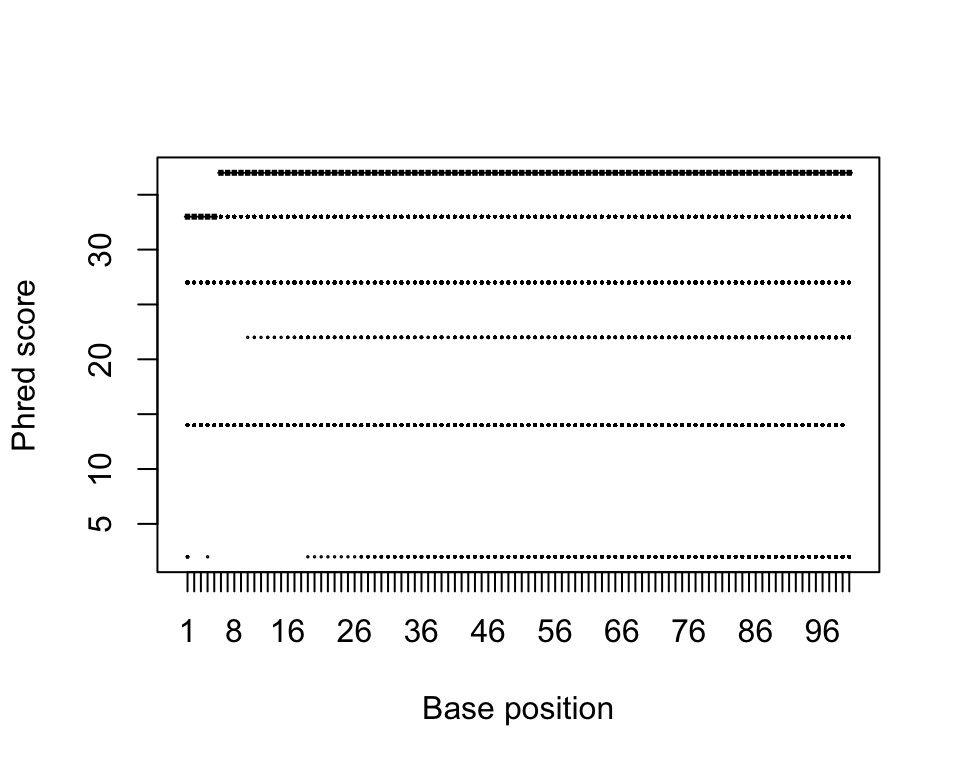
\includegraphics{bookdown-RNA-seq-protocol_files/figure-latex/unnamed-chunk-12-1.pdf}

\textbf{Align and count reads TIMING \textasciitilde{}6 min per library}

\textbf{Step 4}\\
Map sequence reads to mouse genome GRCm38/mm10. It is recommended to provide gene annotation to the read mapping. Mapped reads are saved to BAM files and a mapping summary is returned to R after read mapping is completed.

\begin{Shaded}
\begin{Highlighting}[]
\NormalTok{align.outfiles <-}\StringTok{ }\KeywordTok{paste}\NormalTok{(targets}\OperatorTok{$}\NormalTok{Sample, }\StringTok{"bam"}\NormalTok{, }\DataTypeTok{sep =} \StringTok{"."}\NormalTok{)}
\NormalTok{align.summary <-}
\StringTok{  }\KeywordTok{align}\NormalTok{(}
    \StringTok{"mm10_reference"}\NormalTok{,}
\NormalTok{    targets}\OperatorTok{$}\NormalTok{Library,}
    \DataTypeTok{output_file =}\NormalTok{ align.outfiles,}
    \DataTypeTok{nthreads =} \DecValTok{10}\NormalTok{,}
    \DataTypeTok{useAnnotation =} \OtherTok{TRUE}\NormalTok{,}
    \DataTypeTok{annot.inbuilt =} \StringTok{"mm10"}
\NormalTok{  )}
\NormalTok{align.summary}
\end{Highlighting}
\end{Shaded}

\textbf{Step 5}\\
Assign reads to overlapping genes and generate an R object that contains a count table, gene annotation and counting summary. The count table contains number of reads assigned to each gene in each library. The gene annotation includes Entrez gene identifier, chromosomal coordinates of gene exons and gene length (total number of non-overlapping exonic bases each gene has). The counting summary gives the number of successfully assigned reads in each library and also numbers of reads that failed to be assigned due to filtering. The `Status' column in this summary includes a `Assigned' category and also multiple `Unassigned' categories corresponding to different read filters used in counting.

\begin{Shaded}
\begin{Highlighting}[]
\NormalTok{counts.gene <-}\StringTok{ }\KeywordTok{featureCounts}\NormalTok{(align.outfiles, }\StringTok{"mm10"}\NormalTok{, }\DataTypeTok{nthreads =} \DecValTok{10}\NormalTok{)}
\NormalTok{counts.gene}\OperatorTok{$}\NormalTok{stat}
\end{Highlighting}
\end{Shaded}

\textbf{Save R data and switch from the UNIX server to a personal computer TIMING \textless{} 1 min}

\textbf{(Steps 6 and 7 can be skipped if you run the protocol using `RStudio (2672)' or laptop only)}

\textbf{Step 6 (optional)}\\

Save all generated R objects to a file and then copy the file to your personal computer.

\begin{Shaded}
\begin{Highlighting}[]
\KeywordTok{save.image}\NormalTok{(}\StringTok{"Counts.rdata"}\NormalTok{)}
\end{Highlighting}
\end{Shaded}

\textbf{Step 7 (optional)}\\

Launch R on your personal computer and load R objects from the copied file.

\begin{Shaded}
\begin{Highlighting}[]
\KeywordTok{load}\NormalTok{(}\StringTok{"Counts.rdata"}\NormalTok{)}
\end{Highlighting}
\end{Shaded}

\textbf{Perform differential expression analysis TIMING \textless{} 1 min}

\textbf{Step 8}\\

Load required libraries.

\begin{Shaded}
\begin{Highlighting}[]
\KeywordTok{library}\NormalTok{(limma)}
\KeywordTok{library}\NormalTok{(edgeR)}
\KeywordTok{library}\NormalTok{(statmod)}
\KeywordTok{suppressMessages}\NormalTok{(}\KeywordTok{library}\NormalTok{(org.Mm.eg.db))}
\end{Highlighting}
\end{Shaded}

\textbf{Step 9}\\

Create a design matrix.

\begin{Shaded}
\begin{Highlighting}[]
\NormalTok{ct <-}\StringTok{ }\KeywordTok{factor}\NormalTok{(targets}\OperatorTok{$}\NormalTok{CellType)}
\NormalTok{design <-}\StringTok{ }\KeywordTok{model.matrix}\NormalTok{(}\OperatorTok{~}\DecValTok{0} \OperatorTok{+}\StringTok{ }\NormalTok{ct)}
\KeywordTok{colnames}\NormalTok{(design) <-}\StringTok{ }\KeywordTok{levels}\NormalTok{(ct)}
\end{Highlighting}
\end{Shaded}

\textbf{Step 10}\\

Map Entrez gene identifiers to gene symbols and create an R object containing annotation data for each gene. The annotation data include Entrez gene identifier, gene symbol and gene length.

\begin{Shaded}
\begin{Highlighting}[]
\NormalTok{tmp <-}\StringTok{ }\NormalTok{org.Mm.egSYMBOL}
\NormalTok{entrez_symbol <-}\StringTok{ }\KeywordTok{as.list}\NormalTok{(tmp[}\KeywordTok{mappedkeys}\NormalTok{(tmp)])}
\NormalTok{entrez_symbol <-}\StringTok{ }\KeywordTok{sapply}\NormalTok{(entrez_symbol, }\ControlFlowTok{function}\NormalTok{(x)}
\NormalTok{  x[}\DecValTok{1}\NormalTok{])}
\NormalTok{genes <-}\StringTok{ }\NormalTok{counts.gene}\OperatorTok{$}\NormalTok{annotation}\OperatorTok{$}\NormalTok{GeneID}
\NormalTok{m <-}\StringTok{ }\KeywordTok{match}\NormalTok{(genes, }\KeywordTok{names}\NormalTok{(entrez_symbol))}
\NormalTok{genes <-}\StringTok{ }\KeywordTok{data.frame}\NormalTok{(}
  \DataTypeTok{EntrezID =}\NormalTok{ genes,}
  \DataTypeTok{Symbol =}\NormalTok{ entrez_symbol[m],}
  \DataTypeTok{Length =}\NormalTok{ counts.gene}\OperatorTok{$}\NormalTok{annotation}\OperatorTok{$}\NormalTok{Length,}
  \DataTypeTok{stringsAsFactors =} \OtherTok{FALSE}
\NormalTok{)}
\end{Highlighting}
\end{Shaded}

\textbf{Step 11}\\

Remove from analysis those genes that did not express, or expressed at a very low level, in all cell types. Here we require a gene to have a CPM value greater than 0.5 in at least two libraries to be included in the subsequent analysis. The reason we require at least two libraries is because there are two biological replicates generated for each sample in this dataset.

\begin{Shaded}
\begin{Highlighting}[]
\NormalTok{keep <-}\StringTok{ }\KeywordTok{rowSums}\NormalTok{(}\KeywordTok{cpm}\NormalTok{(counts.gene}\OperatorTok{$}\NormalTok{counts) }\OperatorTok{>}\StringTok{ }\FloatTok{0.5}\NormalTok{) }\OperatorTok{>=}\StringTok{ }\DecValTok{2}
\KeywordTok{sum}\NormalTok{(keep)}
\end{Highlighting}
\end{Shaded}

\begin{verbatim}
## [1] 11969
\end{verbatim}

\textbf{Step 12}\\
Transform count data to log2-cpm, estimate the mean-variance relationship and compute observation-level weights. Log2-cpm expression values of genes are then normalized using the quantile method and converted to log2-rpkm (log2 reads per kilobases of exons per million reads) values.

\begin{Shaded}
\begin{Highlighting}[]
\NormalTok{y <-}
\StringTok{  }\KeywordTok{voom}\NormalTok{(counts.gene}\OperatorTok{$}\NormalTok{counts[keep, ], design, }\DataTypeTok{normalize.method =} \StringTok{"quantile"}\NormalTok{)}
\NormalTok{y}\OperatorTok{$}\NormalTok{genes <-}\StringTok{ }\NormalTok{genes[keep, ]}
\NormalTok{y}\OperatorTok{$}\NormalTok{E <-}\StringTok{ }\NormalTok{y}\OperatorTok{$}\NormalTok{E }\OperatorTok{-}\StringTok{ }\KeywordTok{log2}\NormalTok{(y}\OperatorTok{$}\NormalTok{genes}\OperatorTok{$}\NormalTok{Length }\OperatorTok{/}\StringTok{ }\DecValTok{1000}\NormalTok{)}
\end{Highlighting}
\end{Shaded}

\textbf{Step 13}\\
Cluster samples via multidimensional scaling.

\begin{Shaded}
\begin{Highlighting}[]
\KeywordTok{plotMDS}\NormalTok{(y, }\DataTypeTok{labels=}\NormalTok{targets}\OperatorTok{$}\NormalTok{CellType)}
\end{Highlighting}
\end{Shaded}

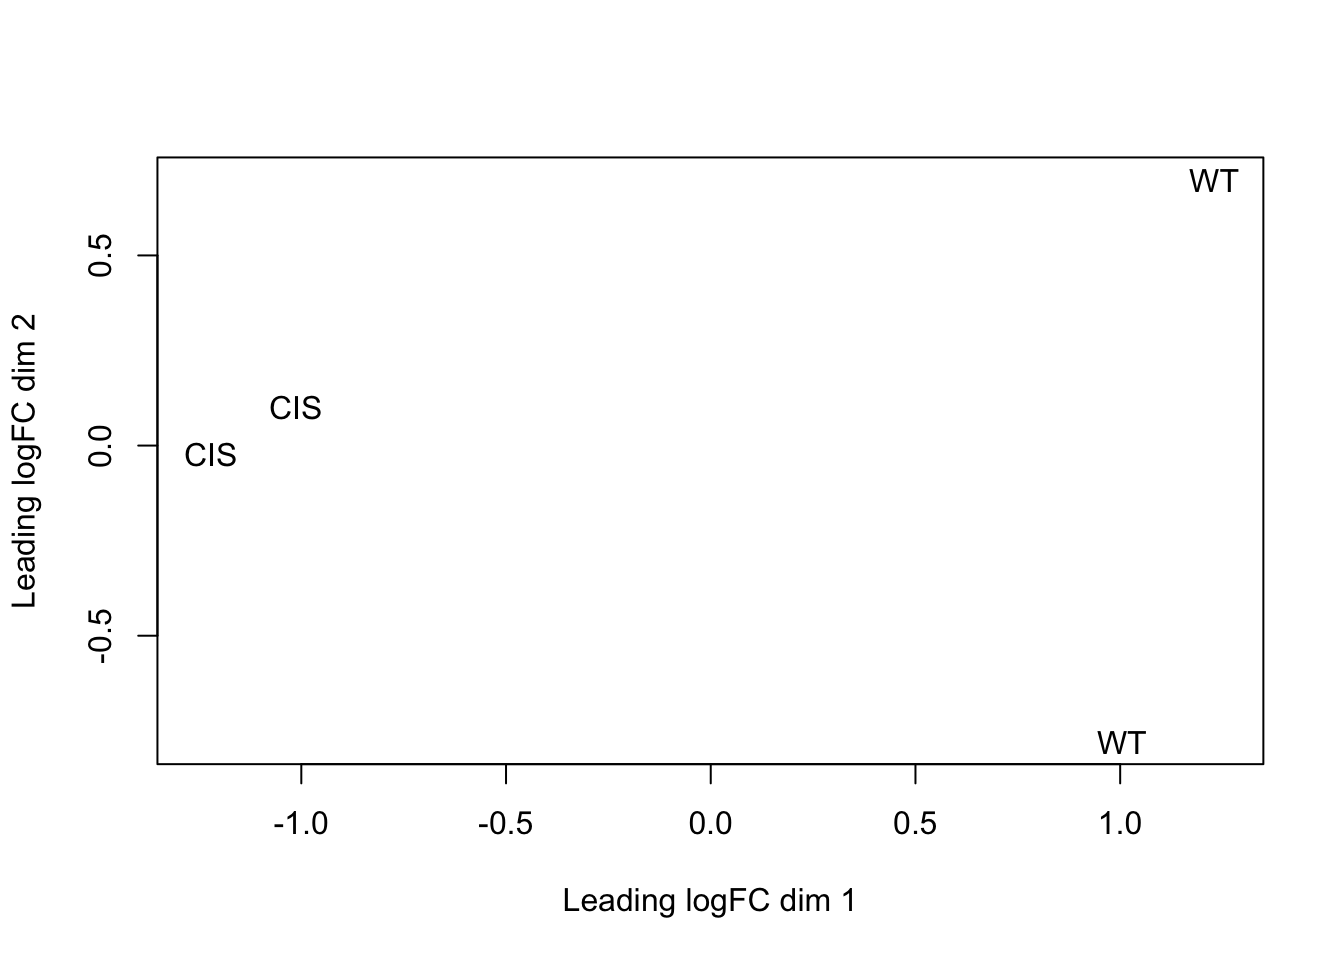
\includegraphics{bookdown-RNA-seq-protocol_files/figure-latex/unnamed-chunk-22-1.pdf}

\textbf{Step 14}\\

Fit linear models to genes and perform statistical testing to discover differentially expressed genes. A contrast matrix is constructed to specify the comparisons between samples. The empirical Bayes moderated t-statistic is used to assess the differential expression of genes. A FDR (false discovery rate) cutoff is applied for calling differentially expressed genes. For this analysis, an FDR cutoff of 0.05 was applied (default cutoff value in decideTests()).

\begin{Shaded}
\begin{Highlighting}[]
\NormalTok{fit <-}\StringTok{ }\KeywordTok{lmFit}\NormalTok{(y, design)}
\NormalTok{contr <-}\StringTok{ }\KeywordTok{makeContrasts}\NormalTok{(}\DataTypeTok{CISvsWT =}\NormalTok{ CIS }\OperatorTok{-}\StringTok{ }\NormalTok{WT, }\DataTypeTok{levels =}\NormalTok{ design)}
\NormalTok{fit.contr <-}\StringTok{ }\KeywordTok{eBayes}\NormalTok{(}\KeywordTok{contrasts.fit}\NormalTok{(fit, contr))}
\NormalTok{dt <-}\StringTok{ }\KeywordTok{decideTests}\NormalTok{(fit.contr)}
\KeywordTok{summary}\NormalTok{(dt)}
\end{Highlighting}
\end{Shaded}

\begin{verbatim}
##        CISvsWT
## Down      1662
## NotSig    8788
## Up        1519
\end{verbatim}

\textbf{Step 15}\\

Display top 10 most differentially expressed genes:

\begin{Shaded}
\begin{Highlighting}[]
\KeywordTok{options}\NormalTok{(}\DataTypeTok{digits=}\DecValTok{2}\NormalTok{)}
\KeywordTok{topTable}\NormalTok{(fit.contr)}
\end{Highlighting}
\end{Shaded}

\begin{verbatim}
##        EntrezID           Symbol Length logFC AveExpr   t P.Value adj.P.Val
## 12700     12700             Cish   2161  -3.5   4.705 -27 2.1e-08   7.4e-05
## 69368     69368            Wdfy1   4714  -2.6   1.999 -21 1.6e-07   3.1e-04
## 21638     21638            Trgv4    419   3.8   3.666  17 5.9e-07   8.8e-04
## 436468   436468 Trav15d-1-dv6d-1    349   4.2   3.098  17 4.8e-07   8.1e-04
## 22290     22290              Uty   5228 -11.0  -2.841 -31 9.7e-09   7.4e-05
## 26908     26908          Eif2s3y   1767 -12.2  -0.086 -27 2.4e-08   7.4e-05
## 26900     26900            Ddx3y   4640 -11.5  -1.825 -27 2.5e-08   7.4e-05
## 20592     20592            Kdm5d   5471 -10.6  -2.515 -25 4.0e-08   9.6e-05
## 59310     59310            Myl10    880   2.6   3.140  14 2.1e-06   2.3e-03
## 13508     13508            Dscam   7481  -2.3   0.022 -14 2.3e-06   2.3e-03
##           B
## 12700  10.1
## 69368   8.2
## 21638   6.6
## 436468  6.3
## 22290   6.1
## 26908   6.0
## 26900   6.0
## 20592   5.8
## 59310   5.7
## 13508   5.6
\end{verbatim}

\textbf{Step 16}\\

Save all differentially expressed genes to a file and all other results for further downstream analysis.

\begin{Shaded}
\begin{Highlighting}[]
\NormalTok{de.genes <-}\StringTok{ }\KeywordTok{topTable}\NormalTok{(fit.contr, }\DataTypeTok{coef=}\StringTok{"CISvsWT"}\NormalTok{, }\DataTypeTok{p.value=}\FloatTok{0.05}\NormalTok{, }\DataTypeTok{n=}\OtherTok{Inf}\NormalTok{)}
\KeywordTok{write.csv}\NormalTok{(de.genes, }\DataTypeTok{file=}\StringTok{"DE_genes.csv"}\NormalTok{, }\DataTypeTok{row.names=}\OtherTok{FALSE}\NormalTok{)}
\end{Highlighting}
\end{Shaded}

\begin{Shaded}
\begin{Highlighting}[]
\CommentTok{#save differential expression results}
\KeywordTok{save}\NormalTok{(fit,fit.contr,dt,de.genes,y,}\DataTypeTok{file =} \StringTok{"DE_results.RData"}\NormalTok{)}
\end{Highlighting}
\end{Shaded}

\hypertarget{more-details-on-the-protocol}{%
\chapter{More details on the protocol}\label{more-details-on-the-protocol}}

\hypertarget{sequencing-quality}{%
\section{Sequencing quality}\label{sequencing-quality}}

Sequencing output from a sequencer is stored in one or more FASTQ-format files. Each FASTQ
file contains nucleotide sequences and sequencing quality strings for the reads generated from a
library. The quality string for a read has the same length as the read sequence and each letter in the string encodes the sequencing quality score of the corresponding read base. The ASCII code of a letter is equal to the Phred quality score of the read base plus an integer offset.
A Phred quality score denotes the sequencing quality of a read base. It is computed as −10 x log10P, where \emph{P} is the probability that a read base is incorrectly called

The \emph{qualityScores()} function in \textbf{Rsubread} extracts quality strings from a FASTQ file and returns the Phred scores in a data matrix object in which rows are reads and columns are base positions. Distribution of Phred scores at each base position can be viewed by using the \emph{boxplot()} function. For reads generated by the popular Illumina sequencers such as HiSeq and NextSeq, sequencing quality is usually lower at the two ends of the read (particular at the 3' end) compared to the middle part of the read. The vast majority of read bases in a FASTQ file are expected to have a Phred score greater than 13 (corresponding to \emph{P} value of 0.05). Fig. 2 shows the boxplots of quality scores in a library that was sequenced in 2015 by an Illumina HiSeq 2000 sequencer. The boxplots show that this dataset has a high sequencing quality.

Box 1 \textbar{} The Simplified Annotation Format (SAF)

\begin{verbatim}
 The Simplified Annotation Format is defined in Rsubread and this format is used by
 featureCounts to counts reads to genes or other genomic features. This format only
 includes five compulsory columns: ‘GeneID’, ‘Chr’, ‘Start’, ‘End’ and
 ‘Strand’. Below is an example of SAF annotation for two RefSeq genes with Entrez
 gene identifiers 497097 and 100503874.
 GeneID    Chr  Start   End     Strand**
 497097    chr1 3204563 3207049  -
 497097    chr1 3411783 3411982  -
 497097    chr1 3660633 3661579  -
 100503874 chr1 3637390 3640590  -
 100503874 chr1 3648928 3648985  -
 Gene identifiers included in the column ‘GeneID’ can be integer numbers (eg. Entrez gene   identifiers) or character strings (eg. gene symbols).
\end{verbatim}

\hypertarget{gene-annotation}{%
\section{Gene annotation}\label{gene-annotation}}

The Rsubread package contains inbuilt gene annotation for human and mouse, making it convenient to process RNA-seq data generated from human or mouse samples. This annotation was generated based on the NCBI RefSeq gene annotation. In this annotation, overlapping exons from the same gene were merged to form a single exon covering all overlapping exons. The inbuilt annotations can be used in both read counting and read mapping. The inbuilt annotations are in SAF format (Box 1). They can be retrieved using the getInBuiltAnnotation() function in Rsubread.

Alternatively, external gene annotations such as those generated in Ensembl database (9) or
GENCODE database (10) can be used for counting and mapping. Formats of external gene annotation that are accepted by Rsubread functions include GTF and GFF3 (\url{https://genome.ucsc.edu/FAQ/FAQformat.html\#format4}).

\hypertarget{index-building}{%
\section{Index building}\label{index-building}}

An index built for a reference genome contains a large hash table, which stores chromosomal
locations of subreads (16bp mers) extracted from the reference genome. With the hash table,
subreads extracted from a read can be quickly mapped to the genome via a quick search (hashing)
in the table. Candidate mapping locations of the read will then be determined by the voting of
mapped subreads and final mapping location will be determined by further evaluation of candidate
mapping locations.

The index can be built as either a full index or a gapped index. A full index contains subreads
extracted from every base location of the genome, whereas a gapped index contains subreads
extracted from every three bases in the genome. The use of a full index will make read mapping
faster, but it also causes more computer memory to be used. Full index and gapped index can be
further split into blocks. This can reduce memory usage but mapping time will increase on the
other hand. See Box 2 for more information on gapped index and split index.

By default, \emph{buildindex()} constructs a single-block full index for a reference genome. This
allows maximum mapping speed to be achieved. To our knowledge, Rsubread is the only tool that
allows users to tune the amount of memory used to achieve a desired balance between memory
consumption and speed in read mapping. This flexibility allows Rsubread to be run on various
computing platforms.

\hypertarget{read-mapping}{%
\section{Read mapping}\label{read-mapping}}

After an index is successfully built, sequencing reads can then be mapped to the reference genome
via the \emph{align()} function. Reads are mapped via a two-pass procedure. In the first pass, subreads (seeds) are extracted from each read and their locations in the genome are quickly determined by looking up the hash table included in the index. Mapped subreads then `vote' for mapping locations of the read. This \emph{`seed-and-vote'} strategy has been demonstrated to be more efficient and accurate than the conventional \emph{`seed-and-extend'} strategy \citep{Rsubread2019, liao2013subread}. Indels will also be discovered in this step.

In the second pass, reads are re-aligned to the genome to determine their final mapping location
by taking into account indels identified from the first pass. Note that \emph{align()} does not perform full alignment for exon-spanning reads. It only aligns such reads to the exon they most overlap with.

Read bases overlapping other exons in such reads are soft-clipped. However this partial alignment
is sufficient for RNA-seq expression quantification at the gene level because reads can be confidently assigned to one of the exons in the gene. To fully align exon-spanning reads, the \emph{subjunc()} function in \textbf{Rsubread} can be used. \emph{subjunc()} is slower than \emph{align()}, but it is still computationally competitive. \emph{subjunc()} is also a two-pass aligner. However it not only collects indels in its first pass, it also collects exon splicing sites. In its second pass, it will use detected exon splicing sites to further improve the mapping of exon-spanning reads.

\begin{verbatim}
Box 2 | Build an index with less memory usage

A gapped index can be built to reduce the index size. 
Size of a gapped index is only one third of size of the full index. 
Use of a gapped index could save more than 50% of memory used in read mapping. 
During read mapping, the memory contains the index and also other data such as chromosomal sequences, read sequences and intermediate mapping data. 
For human or mouse genome, size of the full index is ~15GB and size of the gapped index is 5GB. 
During read mapping, ~18GB of memory is consumed when full index is used and ~8GB when gapped index is used. 
Below is the command for building a gapped index:
> buildindex("mm10_reference", "mm10.fa", gappedIndex=TRUE)
The full index and gapped index can be split into blocks to further 
control the amount of memory to be used. 
Users can specify the maximum memory allowed and  buildindex() will 
automatically split the index into required number of blocks. 
The index blocks will be loaded to memory sequentially during read mapping. 
The more blocks an index is split into, the smaller the memory required for read mapping. However the read mapping time will also increase. 
The following command builds a full index that is split into multiple blocks to achieve a memory use no more than 4000MB.
> buildindex("mm10_reference", "mm10.fa", indexSplit=TRUE,memory=4000)
\end{verbatim}

\textbf{Rsubread} aligners are the first to use the two-pass strategy to improve the mapping quality
of RNA-seq reads. This strategy has later been adopted by other RNA-seq aligners.
Mapping results from \emph{align()} include both mapped and unmapped reads. The results are
saved to files in BAM or SAM format. Indels identified in the mapping are saved to VCF-format
files. \emph{align()} also returns an \textbf{R} object that contains mapping statistics for each library.

Percentage of successfully mapped reads in a library is affected by multiple factors including
sequencing quality, read length, paired-end or single-end, quality of reference sequences and
aligner setting. For the single-end reads generated from the latest Illumina
HiSeq/NextSeq/NovaSeq sequencers, \emph{align()} typically reports around 80-90 percent of mapped
reads. If paired-end reads are provided, the mapping percentage is expected to be slightly higher.

\hypertarget{read-counting}{%
\section{Read counting}\label{read-counting}}

After read mapping is completed, mapped reads can be counted to genes by \emph{featureCounts()}
function in \textbf{Rsubread}. \emph{featureCounts()} compares chromosomal coordinates of mapped reads with chromosomal coordinates of exons in each gene. \emph{CIGAR} (Concise Idiosyncratic Gapped
Alignment Report) string of each mapped read is analyzed so that read assignment can be done
precisely. \emph{featureCounts()} provides a wide range of counting options. For example, overlap
between a read and an exon can be determined based on the number of overlapping bases, fraction
of overlapping bases and number of non-overlapping bases. Multi-mapping reads can be excluded from counting, or only have their primary alignment counted or have all their alignments counted.

Similarly, for multi-overlapping reads that overlap more than one gene they can be excluded from
counting or be counted to all their overlapping genes.

\textbf{featureCounts()} accepts both name-sorted and location-sorted reads. It can output counting
details for each individual read.

\textbf{featureCounts()} returns an R object that includes a count table, gene annotation and counting statistics. Percentage of successfully assigned reads is affected by many factors including cell type, annotation quality and mRNA purity. The counting percentage could be highly variable between experiments, even for well annotated genomes such as human and mouse genomes. Typically around 50 -- 90 percent of mapped reads are assigned to genes in a mouse experiment. For the RNA-seq data used in this protocol, \textasciitilde{}70 percent of reads were successfully assigned.

\hypertarget{gene-filtering}{%
\section{Gene filtering}\label{gene-filtering}}

Genes that do not express or express at a very low level in all the samples are filtered out from analysis. Such genes are very hard to handle in the statistical testing. Typically \textasciitilde{}50 percent of genes are excluded in the analysis of mouse RNA-seq data. For the RNA-seq data used in this protocol, 58 percent of genes were removed from analysis.

\hypertarget{sample-clustering}{%
\section{Sample clustering}\label{sample-clustering}}

Examining the clustering of samples is a useful way to check the quality of samples. Sample
replicates should cluster together and different sample types should separate from each other.

\hypertarget{statistical-testing-of-differential-expression}{%
\section{Statistical testing of differential expression}\label{statistical-testing-of-differential-expression}}

A rigorous \emph{false discovery rate (FDR)} threshold should be applied when calling differentially
expressed genes. This threshold is usually \emph{0.05}, but it might be relaxed to \emph{0.1} or even \emph{0.15} in some circumstances. The \emph{treat()} function in \textbf{limma} might be considered for testing against a fold change of gene expression.

\hypertarget{downstream-analysis}{%
\chapter{Downstream analysis}\label{downstream-analysis}}

In this chapter we will run through a series of example downstream analyses that can be performed on the identified differentially expressed genes.

\hypertarget{visualisations}{%
\section{Visualisations}\label{visualisations}}

There are a number of ways in which you can visualise your RNA-seq data, while in this chapter we attempt to cover the most commonly ways of visualising your RNA-seq data, this is by no means exhaustive.

\hypertarget{heatmaps}{%
\subsection{Heatmaps}\label{heatmaps}}

Heatmaps are a great way of demonstrating the differences in the expression patterns between different conditions in your dataset. Here we use the \emph{coolmap} function within the \textbf{limma}
package which is an extension of the \emph{heatmap.2} function within the \textbf{gplots} package. The heatmap below shows the expression pattern of the top 100 differentially expressed genes between CIS vs WT.

\begin{Shaded}
\begin{Highlighting}[]
\CommentTok{#load the required package}
\KeywordTok{library}\NormalTok{(limma)}
\KeywordTok{load}\NormalTok{(}\StringTok{"Counts.rdata"}\NormalTok{)}
\KeywordTok{load}\NormalTok{(}\StringTok{"DE_results.RData"}\NormalTok{)}
\NormalTok{heat.data <-}\StringTok{ }\NormalTok{y}\OperatorTok{$}\NormalTok{E[}\KeywordTok{head}\NormalTok{(}\KeywordTok{rownames}\NormalTok{(de.genes), }\DataTypeTok{n =} \DecValTok{100}\NormalTok{), ]}
\KeywordTok{colnames}\NormalTok{(heat.data) <-}\StringTok{ }\NormalTok{targets}\OperatorTok{$}\NormalTok{Sample}
\KeywordTok{rownames}\NormalTok{(heat.data) <-}\StringTok{ }\KeywordTok{head}\NormalTok{(de.genes}\OperatorTok{$}\NormalTok{Symbol, }\DataTypeTok{n =} \DecValTok{100}\NormalTok{)}
\KeywordTok{coolmap}\NormalTok{(}
\NormalTok{  heat.data,}
  \DataTypeTok{margin =} \KeywordTok{c}\NormalTok{(}\DecValTok{5}\NormalTok{, }\DecValTok{4}\NormalTok{),}
  \DataTypeTok{cexCol =} \FloatTok{0.8}\NormalTok{,}
  \DataTypeTok{lhei =} \KeywordTok{c}\NormalTok{(}\FloatTok{0.8}\NormalTok{, }\DecValTok{4}\NormalTok{),}
  \DataTypeTok{cexRow =} \FloatTok{0.6}
\NormalTok{)}
\end{Highlighting}
\end{Shaded}

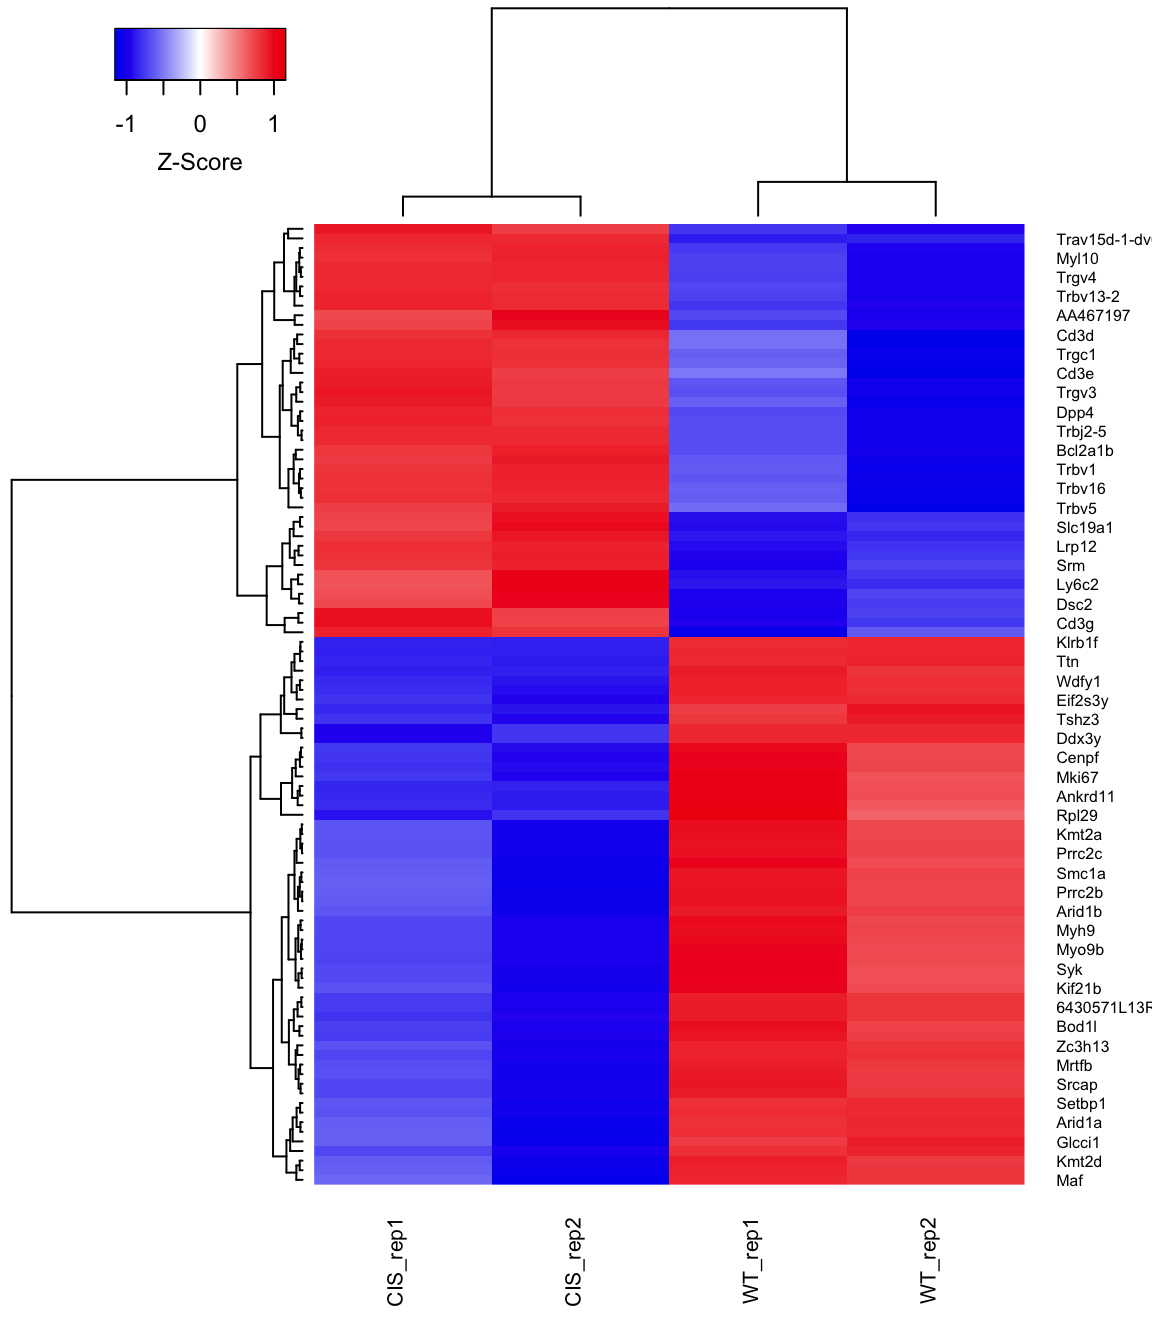
\includegraphics{bookdown-RNA-seq-protocol_files/figure-latex/unnamed-chunk-27-1.pdf}

\hypertarget{mean-difference-plot}{%
\subsection{Mean-difference plot}\label{mean-difference-plot}}

A mean-difference plot or MD-plot is a plot that can be used to show the fold-change differences against the average expression values of all genes used in the analysis. This can be generated easily using the \emph{plotMD} function within the \textbf{limma} package.

\begin{Shaded}
\begin{Highlighting}[]
\KeywordTok{plotMD}\NormalTok{(fit.contr, }\DataTypeTok{column =} \DecValTok{1}\NormalTok{,}\DataTypeTok{status =}\NormalTok{ dt,}\DataTypeTok{cex=}\FloatTok{0.8}\NormalTok{)}
\end{Highlighting}
\end{Shaded}

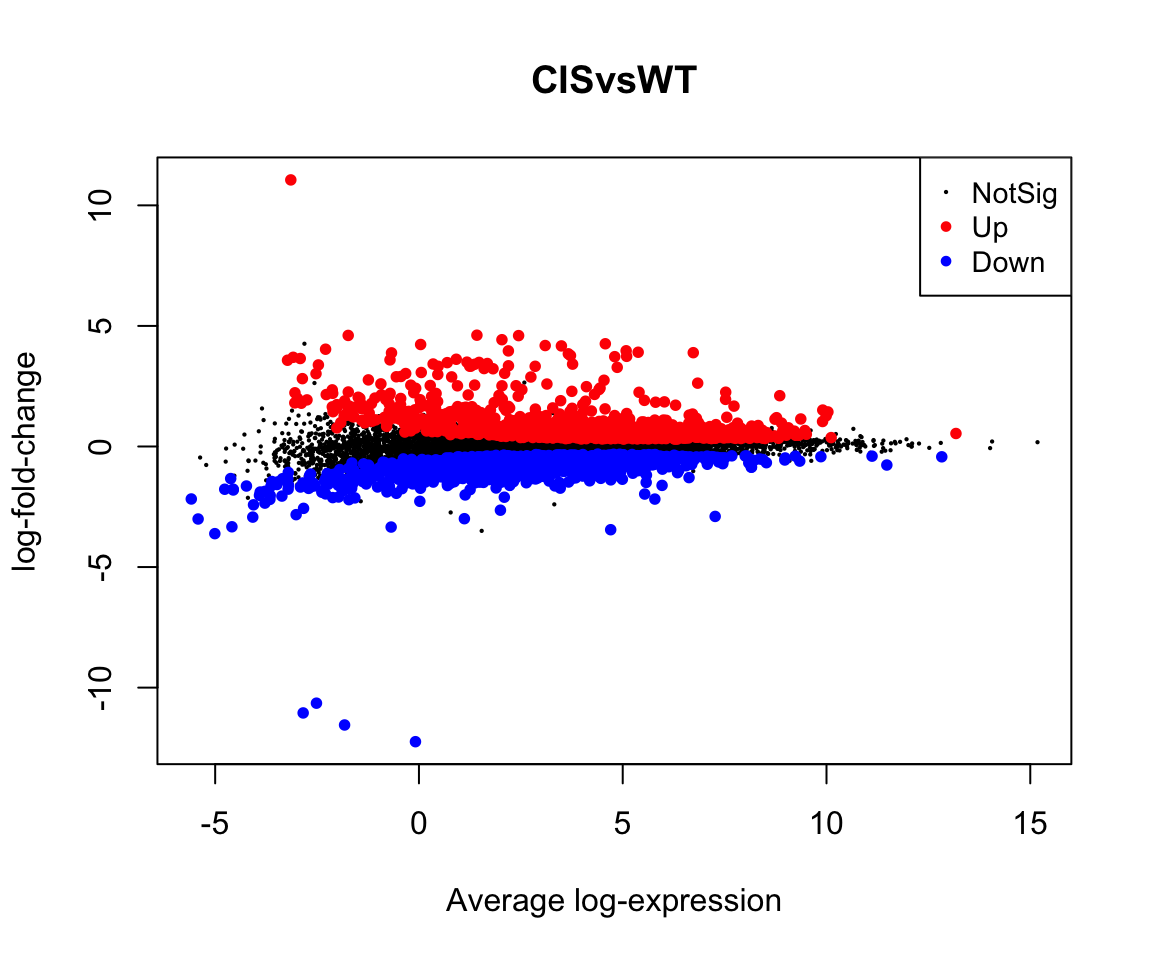
\includegraphics{bookdown-RNA-seq-protocol_files/figure-latex/unnamed-chunk-28-1.pdf}

\hypertarget{volcano-plot}{%
\subsection{Volcano plot}\label{volcano-plot}}

A volcano plot shows the relationship between the log fold-change on the x-axis and a measure of statistical significance on the y-axis. The measure of significance can be -log(p-value) or the B-statistics. Here, we will use the \emph{volcanoplot} function within the \textbf{limma} package.In the volcano plot below, differentially expressed genes are highlighted with red for up-regulated and blue for down-regulated genes.

\begin{Shaded}
\begin{Highlighting}[]
\CommentTok{#highlight de genes}
\NormalTok{col<-}\KeywordTok{c}\NormalTok{(}\StringTok{"blue"}\NormalTok{,}\StringTok{"black"}\NormalTok{,}\StringTok{"red"}\NormalTok{)[}\KeywordTok{factor}\NormalTok{(dt[,}\StringTok{"CISvsWT"}\NormalTok{])]}
\KeywordTok{volcanoplot}\NormalTok{(fit.contr,}\DataTypeTok{col=}\NormalTok{col)}
\end{Highlighting}
\end{Shaded}

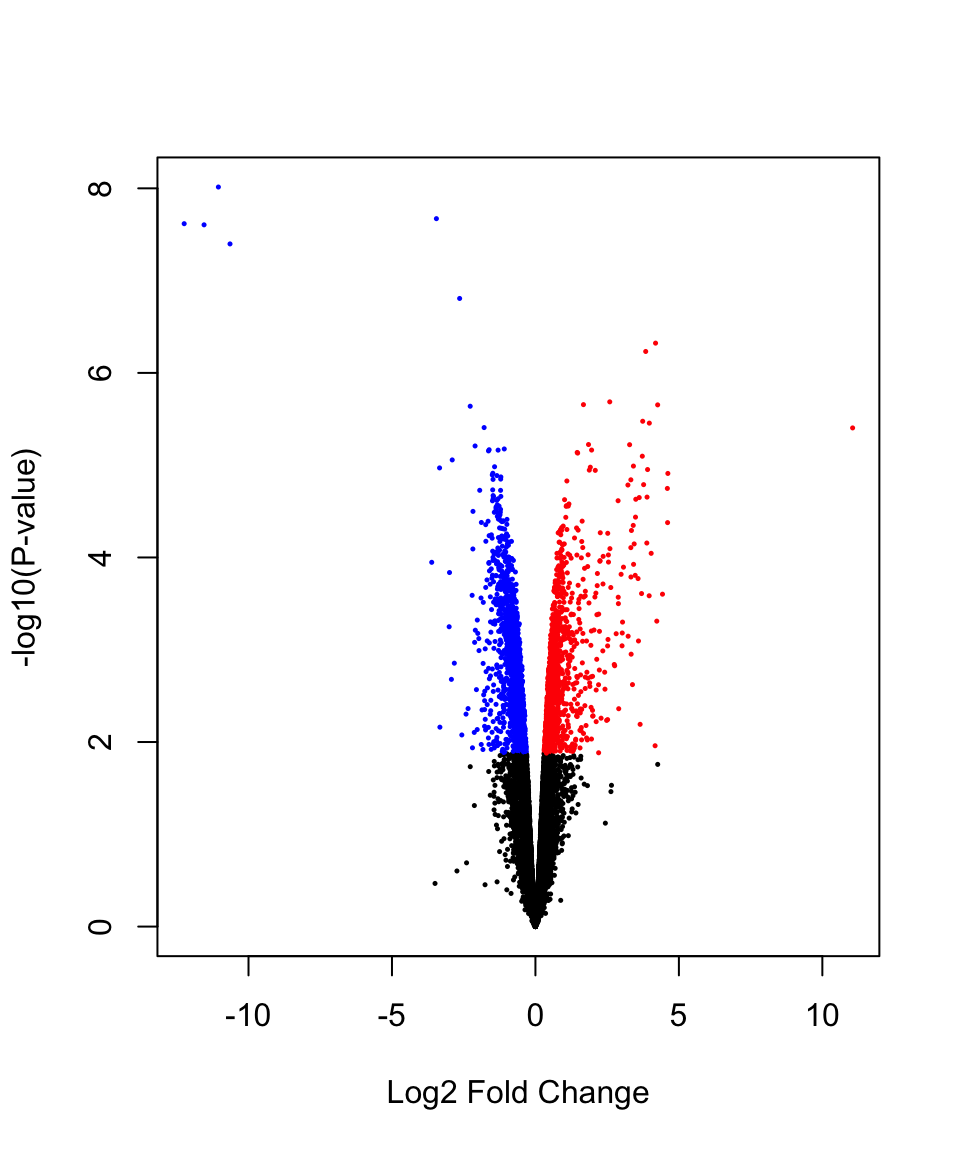
\includegraphics{bookdown-RNA-seq-protocol_files/figure-latex/unnamed-chunk-29-1.pdf}

\hypertarget{gene-ontology-go-and-kegg-enrichment-analysis}{%
\section{Gene Ontology (GO) and KEGG enrichment analysis}\label{gene-ontology-go-and-kegg-enrichment-analysis}}

\hypertarget{gene-ontology}{%
\subsection{Gene Ontology}\label{gene-ontology}}

Gene ontology (\url{http://www.geneontology.org/}) provides a controlled vocabulary for describing biological processes (BP ontology), molecular functions (MF ontology) and cellular components (CC ontology).

The GO ontologies themselves are organism-independent; terms are associated with genes for a specific organism through direct experimentation or through sequence homology with another organism and its GO annotation.

Terms are related to other terms through parent-child relationships in a directed acylic graph.

You can use enrichment analysis as another way of drawing conclusions from your set of differentially expressed genes.

\begin{Shaded}
\begin{Highlighting}[]
\NormalTok{enrich.pvalue<-}\FloatTok{0.00001}
\end{Highlighting}
\end{Shaded}

Here, we use the \emph{goana} function within the \textbf{limma} package to test for enrichment of differentially expressed genes between the CIS vs WT. Note that the \emph{p-values} returned by \emph{goana} are \textbf{unadjusted for multiple testing}. It is therfore, advisable that if the results are to be published, only terms with very small p-values should be included. For instance, in the example below, only terms with a p-value \textless{} \ensuremath{10^{-5}} are retained.

\begin{Shaded}
\begin{Highlighting}[]
\ControlFlowTok{if}\NormalTok{(}\OperatorTok{!}\KeywordTok{requireNamespace}\NormalTok{(}\StringTok{"GO.db"}\NormalTok{))}
\NormalTok{  BiocManager}\OperatorTok{::}\KeywordTok{install}\NormalTok{(}\StringTok{"GO.db"}\NormalTok{)}
\KeywordTok{library}\NormalTok{(GO.db)}
\NormalTok{go.rst<-}\KeywordTok{goana}\NormalTok{(fit.contr,}\DataTypeTok{coef =} \DecValTok{1}\NormalTok{,}\DataTypeTok{FDR =} \FloatTok{0.05}\NormalTok{,}\DataTypeTok{species=}\StringTok{"Mm"}\NormalTok{)}
\CommentTok{#order enriched terms by p-value}
\NormalTok{go.rst<-go.rst[}\KeywordTok{with}\NormalTok{(go.rst,P.Up}\OperatorTok{<}\NormalTok{enrich.pvalue}\OperatorTok{|}\NormalTok{P.Down}\OperatorTok{<}\NormalTok{enrich.pvalue),]}
\NormalTok{go.rst<-}\KeywordTok{topGO}\NormalTok{(go.rst,}\DataTypeTok{number =} \OtherTok{Inf}\NormalTok{)}
\KeywordTok{topGO}\NormalTok{(go.rst)}
\end{Highlighting}
\end{Shaded}

\begin{verbatim}
##                                                              Term Ont    N  Up
## GO:0050794                         regulation of cellular process  BP 6084 593
## GO:0050789                       regulation of biological process  BP 6343 628
## GO:0065007                                  biological regulation  BP 6647 675
## GO:0048522                positive regulation of cellular process  BP 3439 335
## GO:0005515                                        protein binding  MF 5634 584
## GO:0048518              positive regulation of biological process  BP 3697 368
## GO:0060255          regulation of macromolecule metabolic process  BP 3917 361
## GO:0032501                       multicellular organismal process  BP 3570 335
## GO:0048856                       anatomical structure development  BP 3061 287
## GO:0019222                        regulation of metabolic process  BP 4221 404
## GO:0005488                                                binding  MF 7993 876
## GO:0032502                                  developmental process  BP 3334 319
## GO:0031323               regulation of cellular metabolic process  BP 3857 361
## GO:0048731                                     system development  BP 2484 228
## GO:0007275                     multicellular organism development  BP 2804 261
## GO:0016043                        cellular component organization  BP 3824 409
## GO:0006996                                 organelle organization  BP 2732 266
## GO:0010604 positive regulation of macromolecule metabolic process  BP 2214 224
## GO:0051171      regulation of nitrogen compound metabolic process  BP 3590 321
## GO:0080090                regulation of primary metabolic process  BP 3689 332
##            Down P.Up  P.Down
## GO:0050794 1177    1 5.2e-68
## GO:0050789 1206    1 6.1e-66
## GO:0065007 1233    1 6.5e-61
## GO:0048522  746    1 4.5e-50
## GO:0005515 1069    1 6.7e-50
## GO:0048518  779    1 1.6e-47
## GO:0060255  808    1 7.0e-46
## GO:0032501  754    1 1.0e-45
## GO:0048856  673    1 1.3e-45
## GO:0019222  853    1 1.4e-45
## GO:0005488 1360    1 1.5e-45
## GO:0032502  716    1 2.1e-45
## GO:0031323  796    1 6.2e-45
## GO:0048731  575    1 1.4e-44
## GO:0007275  628    1 1.7e-44
## GO:0016043  789    1 2.7e-44
## GO:0006996  607    1 2.5e-41
## GO:0010604  518    1 1.4e-40
## GO:0051171  738    1 1.8e-39
## GO:0080090  753    1 2.2e-39
\end{verbatim}

A simple way to visualise the enrichment results is through a bar plot as shown below which shows the top 10 enriched terms

\begin{Shaded}
\begin{Highlighting}[]
\NormalTok{top.up <-}\StringTok{ }\KeywordTok{head}\NormalTok{(go.rst[}\KeywordTok{order}\NormalTok{(go.rst}\OperatorTok{$}\NormalTok{P.Up, }\DataTypeTok{decreasing =}\NormalTok{ F), ], }\DataTypeTok{n =} \DecValTok{10}\NormalTok{)}
\NormalTok{top.down <-}\StringTok{ }\KeywordTok{head}\NormalTok{(go.rst[}\KeywordTok{order}\NormalTok{(go.rst}\OperatorTok{$}\NormalTok{P.Down, }\DataTypeTok{decreasing =}\NormalTok{ F), ], }\DataTypeTok{n =} \DecValTok{10}\NormalTok{)}
\NormalTok{bar.data <-}
\StringTok{  }\KeywordTok{rbind}\NormalTok{(}
    \KeywordTok{data.frame}\NormalTok{(}
      \DataTypeTok{Term =}\NormalTok{ top.up}\OperatorTok{$}\NormalTok{Term,}
      \DataTypeTok{P.value =}\NormalTok{ top.up}\OperatorTok{$}\NormalTok{P.Up,}
      \DataTypeTok{Dir =} \StringTok{"up"}
\NormalTok{    ),}
    \KeywordTok{data.frame}\NormalTok{(}
      \DataTypeTok{Term =}\NormalTok{ top.down}\OperatorTok{$}\NormalTok{Term,}
      \DataTypeTok{P.value =}\NormalTok{ top.down}\OperatorTok{$}\NormalTok{P.Down,}
      \DataTypeTok{Dir =} \StringTok{"down"}
\NormalTok{    )}
\NormalTok{  )}
\NormalTok{bar.data <-}\StringTok{ }\NormalTok{bar.data[}\KeywordTok{order}\NormalTok{(bar.data}\OperatorTok{$}\NormalTok{P.value, }\DataTypeTok{decreasing =}\NormalTok{ F), ]}
\KeywordTok{par}\NormalTok{(}\DataTypeTok{mai =} \KeywordTok{c}\NormalTok{(}\FloatTok{0.8}\NormalTok{, }\DecValTok{2}\NormalTok{, }\FloatTok{0.5}\NormalTok{, }\FloatTok{0.5}\NormalTok{))}
\NormalTok{bb<-}\KeywordTok{barplot}\NormalTok{(}
  \OperatorTok{-}\KeywordTok{log10}\NormalTok{(bar.data}\OperatorTok{$}\NormalTok{P.value),}
  \DataTypeTok{horiz =}\NormalTok{ T,}
  \DataTypeTok{xlab =} \StringTok{" -log10(p-value)"}\NormalTok{,}
  \DataTypeTok{cex.names =} \FloatTok{0.5}\NormalTok{,}
  \DataTypeTok{col =} \KeywordTok{c}\NormalTok{(}\StringTok{"red"}\NormalTok{,}\StringTok{"blue"}\NormalTok{)[}\KeywordTok{factor}\NormalTok{(bar.data}\OperatorTok{$}\NormalTok{Dir)]}
\NormalTok{)}
\KeywordTok{axis}\NormalTok{(}\DecValTok{2}\NormalTok{,}\DataTypeTok{line =} \FloatTok{-0.8}\NormalTok{,}\DataTypeTok{at=}\NormalTok{bb,}\DataTypeTok{labels =}\NormalTok{ bar.data}\OperatorTok{$}\NormalTok{Term,}\DataTypeTok{tick =}\NormalTok{ F,}\DataTypeTok{las=}\DecValTok{2}\NormalTok{,}\DataTypeTok{cex.axis=}\FloatTok{0.5}\NormalTok{)}
\end{Highlighting}
\end{Shaded}

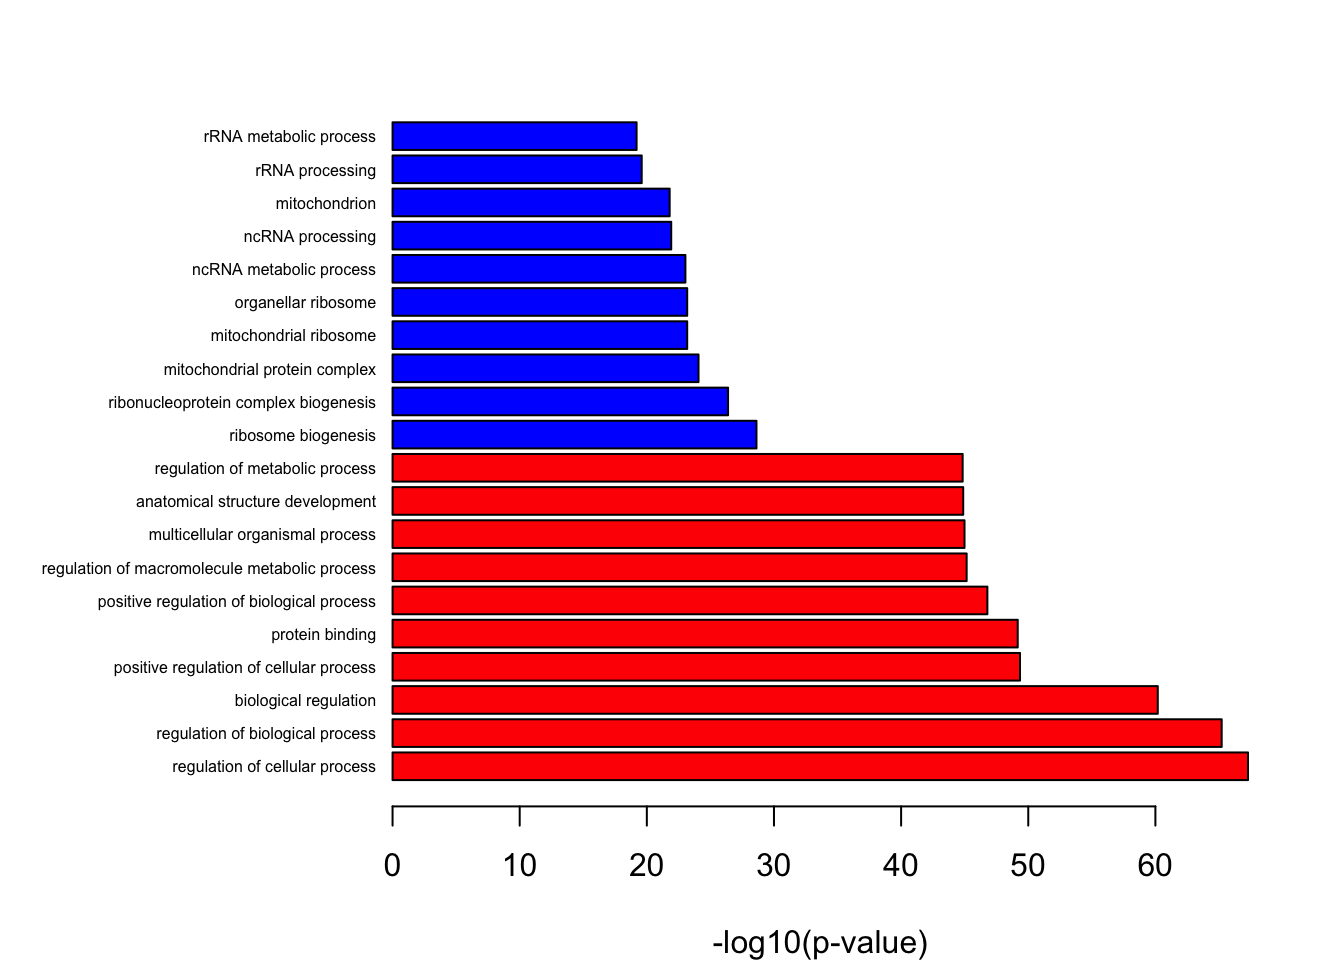
\includegraphics{bookdown-RNA-seq-protocol_files/figure-latex/unnamed-chunk-32-1.pdf}

\textbf{Add gene information (optional)}

Sometimes you may want to know what genes are enriched in each of the terms, this section allows you to add gene details.

\begin{Shaded}
\begin{Highlighting}[]
\KeywordTok{library}\NormalTok{(org.Mm.eg.db)}
\NormalTok{go.EntrezID <-}\StringTok{ }\KeywordTok{as.list}\NormalTok{(org.Mm.egGO2ALLEGS)}
\NormalTok{go.rst <-}\StringTok{ }\NormalTok{tibble}\OperatorTok{::}\KeywordTok{rownames_to_column}\NormalTok{(go.rst, }\DataTypeTok{var =} \StringTok{"GO.ID"}\NormalTok{)}

\CommentTok{#Add gene details}
\NormalTok{go.rst}\OperatorTok{$}\NormalTok{Genes.Up <-}\StringTok{ }\KeywordTok{unlist}\NormalTok{(}\KeywordTok{lapply}\NormalTok{(go.rst}\OperatorTok{$}\NormalTok{GO.ID, }\ControlFlowTok{function}\NormalTok{(x) \{}
\NormalTok{  xx <-}\StringTok{ }\NormalTok{go.EntrezID[[x]]}
  \ControlFlowTok{if}\NormalTok{ (}\KeywordTok{is.null}\NormalTok{(xx) }\OperatorTok{|}
\StringTok{      }\KeywordTok{with}\NormalTok{(go.rst[go.rst}\OperatorTok{$}\NormalTok{GO.ID }\OperatorTok{==}\StringTok{ }\NormalTok{x,], Up }\OperatorTok{==}\StringTok{ }\DecValTok{0} \OperatorTok{|}
\StringTok{           }\NormalTok{P.Up }\OperatorTok{>}\StringTok{ }\NormalTok{enrich.pvalue))}
    \KeywordTok{return}\NormalTok{(}\StringTok{"-"}\NormalTok{)}
\NormalTok{  x <-}\StringTok{ }\KeywordTok{rownames}\NormalTok{(dt[}\KeywordTok{rownames}\NormalTok{(dt) }\OperatorTok\StringTok{ }\NormalTok{xx }\OperatorTok{&}\StringTok{ }\NormalTok{dt }\OperatorTok{==}\StringTok{ }\DecValTok{1}\NormalTok{,])}
\NormalTok{  x <-}
\StringTok{    }\KeywordTok{paste0}\NormalTok{(}\KeywordTok{with}\NormalTok{(fit.contr}\OperatorTok{$}\NormalTok{genes, Symbol[EntrezID }\OperatorTok\StringTok{ }\NormalTok{xx]), }\DataTypeTok{collapse =} \StringTok{"|"}\NormalTok{)}
  \KeywordTok{return}\NormalTok{(x)}
\NormalTok{\}))}

\NormalTok{go.rst}\OperatorTok{$}\NormalTok{Genes.Down <-}\StringTok{ }\KeywordTok{unlist}\NormalTok{(}\KeywordTok{lapply}\NormalTok{(go.rst}\OperatorTok{$}\NormalTok{GO.ID, }\ControlFlowTok{function}\NormalTok{(x) \{}
\NormalTok{  xx <-}\StringTok{ }\NormalTok{go.EntrezID[[x]]}
  \ControlFlowTok{if}\NormalTok{ (}\KeywordTok{is.null}\NormalTok{(xx) }\OperatorTok{|}
\StringTok{      }\KeywordTok{with}\NormalTok{(go.rst[go.rst}\OperatorTok{$}\NormalTok{GO.ID }\OperatorTok{==}\StringTok{ }\NormalTok{x,], Down }\OperatorTok{==}\StringTok{ }\DecValTok{0} \OperatorTok{|}
\StringTok{           }\NormalTok{P.Down }\OperatorTok{>}\StringTok{ }\NormalTok{enrich.pvalue))}
    \KeywordTok{return}\NormalTok{(}\StringTok{"-"}\NormalTok{)}
\NormalTok{  x <-}\StringTok{ }\KeywordTok{rownames}\NormalTok{(dt[}\KeywordTok{rownames}\NormalTok{(dt) }\OperatorTok\StringTok{ }\NormalTok{xx }\OperatorTok{&}\StringTok{ }\NormalTok{dt }\OperatorTok{==}\StringTok{ }\DecValTok{-1}\NormalTok{,])}
\NormalTok{  x <-}
\StringTok{    }\KeywordTok{paste0}\NormalTok{(}\KeywordTok{with}\NormalTok{(fit.contr}\OperatorTok{$}\NormalTok{genes, Symbol[EntrezID }\OperatorTok\StringTok{ }\NormalTok{xx]), }\DataTypeTok{collapse =} \StringTok{"|"}\NormalTok{)}
  \KeywordTok{return}\NormalTok{(x)}
\NormalTok{\}))}
\end{Highlighting}
\end{Shaded}

\bibliography{book.bib,packages.bib,Genome.bib}

\end{document}
